\documentclass{scrartcl}
\usepackage[parfill]{parskip}
\usepackage{graphicx}
\usepackage{amssymb}
\usepackage{amsmath}
\DeclareMathOperator*{\argmax}{arg\,max}
\DeclareMathOperator*{\argmin}{arg\,min}
\usepackage{url}
\usepackage{hyperref}

\begin{document}

\title{Notes}

\maketitle

\begin{abstract}
Some notes about Machine Learning concepts.
\end{abstract}

\section{Maximum Likelihood Estimation (MLE)}
\footnote{\url{https://de.wikipedia.org/wiki/Maximum-Likelihood-Methode}} \footnote{\url{https://towardsdatascience.com/probability-concepts-explained-maximum-likelihood-estimation-c7b4342fdbb1}}
Maximum likelihood estimation is a method that determines values for the parameters of a model. The parameter values are found such that they maximise the likelihood that the process described by the model produced the data that were actually observed.

We first have to decide which model we think best describes the process of generating the data.

Then what we want to calculate is the total probability of observing all of the data, i.e. the joint probability distribution of all observed data points. To do this we would need to calculate some conditional probabilities, which can get very difficult. So it is here that we will make our first assumption. \textit{The assumption is that each data point is generated independently of the others.} This assumption makes the maths much easier. If the events (i.e. the process that generates the data) are independent, then the total probability of observing all of data is the product of observing each data point individually (i.e. the product of the marginal probabilities).

$$f(x_1, \dots, x_n; \theta) = \prod_{i=1}^n f(x_i; \theta)$$
$$L(\theta) = \prod_{i=1}^n f_{\theta}(x_i)$$

We now search for the parameters $\theta$ that maximize the Likelihood-function $L$, i.e. $\theta_{ML} = \argmax_{\theta \in \Theta} L(\theta)$. We can do this by differentiation. All we have to do is find the derivative of the function.

The above expression for the total probability is actually quite a pain to differentiate, so it is almost always simplified by taking the natural logarithm of the expression. This is absolutely fine because the natural logarithm is a monotonically increasing function. This means that if the value on the x-axis increases, the value on the y-axis also increases. This is important because it ensures that the maximum value of the log of the probability occurs at the same point as the original probability function.

$$log(L(\theta)) = log(\prod_{i=1}^n f_{\theta}(x_i)) = \sum_{i=1}^n log(f_{\theta}(x_i))$$

\section{Binary cross entropy}
$$H_p(q) = -\frac{1}{N} \sum_{i=1}^N y_i \cdot log(p(y_i)) + (1-y_i) \cdot (1-p(y_i))$$
where $y_i$ is the true class label and $p(y_i)$ is the predicted probability of $x_i$ coming from the positive class $y=1$. Basically: \textbf{sum of negative logs of predicted true class probabilities} (weighted by number of samples). Look at figure \ref{fig:binary_cross_neg_log} for negative log loss.

\begin{figure}
	\centering
		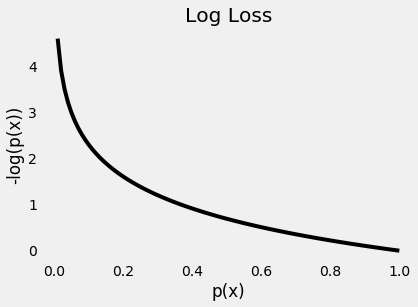
\includegraphics[scale=0.7]{img/binary_cross_neg_log}
	\caption{Negative log loss}
	\label{fig:binary_cross_neg_log}
\end{figure}

\subsection{Diving deeper}
\textbf{Entropy} is a measure of uncertainty associated with a given distribution $q(y)$.

$$H(q) = - \sum_{c=1}^C q(y_c) \cdot log(q(y_c))$$

Example with two classes (and $log$ base $2$):
\begin{itemize}
	\item
		All points from one class: $H(q) = - 1 \cdot log(1) = 0$ $\Rightarrow$ no uncertainty
	\item
		50:50 distribution: $H(q) = -log(0.5) = 1$ $\Rightarrow$ maximum uncertainty
\end{itemize}


\section{Generative Adversarial Networks (GANs)}
\footnote{\url{https://arxiv.org/pdf/1701.00160.pdf}}
\subsection{How do GANs work?}
The basic idea of GANs: set up game between two players. One of them is called \textbf{generator} and creates samples that are intended to come from the same distribution as the training data. The other player is the \textbf{discriminator} who examines samples to determine whether they are real or fake.

Formally, GANs are a structured probabilistic model containing latent variables $z$ and observed variables $x$. 


The two players in the game are represented by two functions, each of which is differentiable both with respect to its inputs and with respect to its parameters.
\begin{itemize}
	\item
		Discriminator: $D$ takes $x$ as input and uses $\theta^{(D)}$ as parameters
	\item
		Generator: $G$ takes $z$ as input and uses $\theta^{(G)}$ as parameters
\end{itemize}

Both players have cost functions that are defined in terms of both players’ parameters.
\begin{itemize}
	\item
		Discriminator: wishes to minimize $J^{(D)}(\theta^{(D)},\theta^{(G)})$ while controlling only $\theta^{(D)}$
	\item
		Generator: wishes to minimize $J^{(G)}(\theta^{(D)},\theta^{(G)})$ while controlling only $\theta^{(G)}$
\end{itemize}


Because each player's cost depends on the other player’s parameters, but each player cannot control the other player’s parameters, this scenario is most straightforward to describe as a game rather than as an optimization problem. . The solution to an optimization problem is a (local) minimum, a point in parameter space where all neighboring points have greater or equal cost. The solution to a game is a Nash equilibrium. . Here, we use the terminology of local differential Nash equilibria
(Ratliff et al., 2013). In this context, a Nash equilibrium is a tuple $(\theta^{(D)},\theta^{(G)})$ that is a local minimum of $J^{(D)}$ w.r.t $\theta^{(D)}$ and a local minimum of $J^{(G)}$ w.r.t $\theta^{(G)}$.

\textbf{The training process.} The training process consists of simultaneous SGD. On each step, two minibatches are sampled: a minibatch of $x$ values from the
dataset and a minibatch of $z$ values drawn from the model’s prior over latent
variables. Then two gradient steps are made simultaneously: one updating $\theta^{(D)}$ to reduce $J^{(D)}$ and one updating $\theta^{(G)}$ to reduce $J^{(G)}$. In both cases, it is possible to use the gradient-based optimization algorithm of your choice. Adam (Kingma and Ba, 2014) is usually a good choice.

\subsection{Cost functions}
Several different cost functions may be used within the GANs framework.

\subsubsection{The discriminators cost, $J^{(D)}$}
The cost used for the discriminator is:
$$J^{(D)}(\theta^{(D)},\theta^{(G)}) = -\frac{1}{2} \mathbb{E}_{x \sim{} p_{data}} log D(x) - \frac{1}{2} \mathbb{E}_z log(1 - D(G(z))).$$

This is just the standard cross-entropy cost that is minimized when training
a standard binary classifier with a sigmoid output. The only difference is that the classifier is trained on two minibatches of data; one coming from the dataset, where the label is 1 for all examples, and one coming from the generator, where the label is 0 for all examples.

\end{document}